%=========================================================================
% (c) Michal Bidlo, Bohuslav Křena, 2008

\iffalse

Způsoby, jak reprezentovat a uchovávat \emph{entity} existuje velké množství. V začátcích herního průmyslu byly \emph{entity} velmi úzce provázány s okolním kódem, ale díky velikosti týmů, které na hrách pracovaly, a relativní jednoduchosti her toto nebyl problém. Avšak s růstem složitosti se začaly používat další přístupy, jako například \emph{objektově orientované programování}, kdy je využíván \emph{polymorfismus} a \emph{dědičnost}. 

Cílem této práce je návrh a implementace knihovny pro dynamickou kompozici objektů, za běhu aplikace. Mezi hlavní požadavky patří \emph{thread-safe}\cite{ThreadSafety} rozhraní, které je možné používat ve vícevláknových aplikacích. Další prioritou je skutečné využití a prospěch z běhu na více vláknech, jednoduchost použití a integrace do již existujících projektů a minimalizace režie.

Práce je rozdělena do čtyř logických celků -- teoretická část\ref{Chap:Theory}, návrh systému\ref{Chap:Design}, implementace\ref{Chap:Implementation}, vyhodnocení a praktická použitelnost výsledné knihovny.

Kapitola \ref{Chap:Theory} se zabývá aktuálním stavem v návrhu \emph{software} a důvody proč je metoda \emph{datově orientované kompozice} důležitá. Jelikož efektivní využití architektury moderních počítačů je stále více důležité, byly při návrhu knihovny použity techniky datově orientovaného návrhu\cite{DataOrientedDesign}, jehož výhody a bližší popis je součástí kapitoly \ref{Chap:DDD}. Další důležitou částí je efektivní využití vícevláknových procesorů, kterým se zabývá kapitola \ref{Chap:Parallelism}.

Kapitola \ref{Chap:Design} obsahuje obecný návrh systému pro dynamickou kompozici, který není závislý na implementačním jazyce. První část \ref{Chap:Overview} obsahuje přehled celého systému, vymezení funkcionality jednotlivých bloků a jejich komunikace. Následují sekce o \emph{komponentech}(\ref{Chap:Component}), \emph{systémech}(\ref{Chap:System}) a \emph{entitách}(\ref{Chap:Entity}), ve kterých je specifikována jejich funkce. Návrhem paralelního přístupu a popis podporovaných možností paralelizace se zabývá sekce \ref{Chap:ParallelismDesign}.

Následuje kapitola \ref{Chap:Implementation}, ve které je popsána implementace výše zmíněného návrhu v jazyce \emph{C++}. První část se zabývá psaním přenositelného kódu v jazyce \emph{C++} a zdůvodnění výběru implementačního jazyka. Následuje popis implementace jednotlivých částí návrhu. Sekce \ref{Chap:CompImpl} obsahuje způsob registrace \emph{komponentů}, definuje, co může být \emph{komponentem} a základní typy datových struktur pro jejich uchovávání. Následuje popis \emph{systémů}, jejich definice a způsob, jakým jsou určeny k používání. Dále je zde shrnuta implementace \emph{entity} a výběr mezi horizontálními a vertikálními \emph{metadaty} s ohledem na paralelizmus. Nakonec je popsána funkce \emph{refresh} a způsoby zajištění parlelního přístupu.

Poslední část se skládá z příkladu využití knihovny v kapitole \ref{Chap:Demo} a vyhodnocení \ref{Chap:Eval}. Knihovna je zhodnocena z pohledu použitelnosti (\ref{Chap:Usability}), výkonosti (\ref{Chap:Performance}) a nakonec porovnána proti vybraným \emph{open-source} knihovnám.

Jelikož se využití \emph{komponentních systémů} začalo objevovat až v posledních letech, neexistuje obecně uznávaný způsob, jak by přesně měl vypadat. Existuje mnoho různých prací na toto téma

Právě tato metoda -- \emph{kompozice} místo \emph{dědičnosti} -- se začíná v herním průmyslu používat stále častěji. Díky celkové neprobádanosti tohoto návrhu existuje mnoho různých způsobů jak by takový systém měl vypadat a jaké části by měl obsahovat.

Tato metoda vzniká z použití tzv. \emph{datově orientovaného návrhu}\cite{DOD}, který se zabývá návrhem aplikací skrz analýzu a transformace dat. Jelikož je tento způsob návrhu stále vcelku nový, existuje mnoho způsobů, jak systém \emph{dynamické kompozice} navrhnout. 

Důležitou vlastností entitního systému založeného na kompozici je právě modularita, která umožňuje ...

Tato metoda vzniká z použití tzv. \emph{datově orientovaného návrhu}\cite{DOD}.

První dokumentované použití se objevuje ve hře \emph{Dungeon Siege}\cite{DungeonSiege} \emph{Tony Hawk}, kdy \emph{Mick West} během několika let transformoval celou hierarchii na právě kompozici z \emph{komponentů}. Následoval po

\fi

\chapter{Úvod}

Díky rostoucím požadavkům na moderní hry -- jak ve složitosti herních principů, tak i věrnosti grafické reprezentace -- se stále zvyšují požadavky na \emph{herní engine}, použitých v jejich tvorbě. Mezi hlavní požadavky patří široké využití v mnoha herních žánrech, možnosti multiplatformního nasazení, efektivní použití dostupného hardware, ale také jednoduchost a efektivita práce ve velkých týmech. Tyto, ale i další problémy řeší návrhový vzor \emph{entity-component-system}, který v základu používá \emph{kompozici} místo \emph{dědičnosti}.

Jelikož je tato metoda vcelku nová, širší využití začíná až v posledních letech, existuje mnoho návrhů, jak by \emph{entitní systém} založený na kompozici měl vypadat. Nejčastěji je návrh rozdělen do tří celků -- \emph{entita}, \emph{komponent} a \emph{systém}. Často se také využívá tzv. \emph{datově orientovaného návrhu}\cite{DOD}, který specifikuje návrh aplikace za použití analýzy vstupních a výstupních dat jednotlivých částí.

Cílem práce je návrh a implementace \emph{entitního systému} založeného na \emph{datově orientované kompozici}. Hlavními požadavky na tento systém jsou: 
\begin{itemize}
	\item Použitelnost ve vícevláknových aplikacích.
	\item Efektivní využití hardwarových prostředků.
	\item Jednoduché rozhraní a integrace do existujících projektů.
\end{itemize}
Mezi další požadavky, z pohledu \emph{herního enginu}, jsou efektivní práce s velkým množstvím \emph{entit}, kde většina z nich nemusí být aktuálně používána a také komunikace mezi jednotlivými \emph{komponenty} a \emph{entitami}.

Práce je rozdělena do čtyř logických celků -- teoretická část, návrh systému, implementace a vyhodnocení. Kapitola \ref{Chap:Theory} popisuje aktuální stav návrhu \emph{software}, primárně z pohledu herního vývoje. Nejdříve zde jsou přiblíženy požadavky na \emph{entitní systémy}. Následuje porovnání aktuálně používaných způsobů reprezentace \emph{entit}, jejich výhody a nevýhody. Závěr obsahuje způsoby využití vícevláknových konfigurací. Kapitola \ref{Chap:Design} zahrnuje kompletní návrh \emph{entitního systému}, který je obecný -- nezávislý na implementačním jazyce. Nejdříve je uveden přehled celého systému, následuje podrobnější popis jeho částí a rozbor různých způsobů řešení. Další kapitola (\ref{Chap:Implementation}) je věnována implementaci v jazyce C++. Následuje kapitola \ref{Chap:Demo}, ve které je předvedena funkčnost systému na návrhu a implementaci demo hry. Poslední kapitola shrnuje výsledný systém z pohledu výkonosti a srovnává jej s podobnými \emph{open-source} knihovnami.

\chapter{Teoretický rozbor}

Tato se věnuje teorii \emph{entitních systémů}, jejich historii a požadavkům na ně kladeným. Dále obsahuje rozbor běžně používaných způsobů reprezentace \emph{entit} a srovnává jejich výhody a nevýhody. Následuje popis vlastního \emph{entitního systému} založeného na kompozici, definice hlavních pojmů -- \emph{entita}, \emph{komponent} a \emph{systém}. Na závěr se věnuje metodám paralelizmu, které jsou dnes používány.

\section{Entitní systémy a jejich historie}

\emph{Entitní systém} je část herního enginu, který zprostředkovává zprávu \emph{entit} -- objektů ve virtuálním světě. Alternativní název, který se také často používá, je \emph{herní objekt} (\emph{Game Object} \cite{UnityGo}). Primární funkcí \emph{entit} je propojení jednotlivých modulů a částí aplikace, které jsou vyvíjeny odděleně -- např. herní logika a simulace fyziky.

\todo{historie}

\section{Požadavky na návrh}

Stále zvyšující se požadavky na složitost herních principů, věrnost grafické reprezentace a velikost virtuálních světů mnohonásobně ztěžují návrh \emph{herních enginů}, na kterých jsou hry stavěny. Dalším problémem je znovupoužitelnost již vytvořených částí, nejen ve stejném projektu, ale stále častěji i v dalších hrách. Z výše zmíněných důvodů vznikají techniky pro organizaci kódu a knihy \emph{návrhových vzorů}\cite{DesignPatterns}\cite{GameDesignPatterns}, které obsahují zkušenosti a prověřené způsoby jak navrhovat \emph{software}. Důležitou vlastností správného návrhu, je také modularita -- oddělení částí systému. Tyto techniky umožňují pracovat velkému množství programátorů na jednom projektu.

Mezi techniky dnes používané patří primárně \emph{objektově orientované návrh}, ale stále častěji také návrh \emph{datově orientovaný}, kterým se zabývá část \ref{Chap:DDD}.

Způsob reprezentace \emph{entit} -- objektů ve virtuálním světě -- je jedním z důležitých rozhodnutí v návrhu \emph{herního enginu}. Entity jsou často používány pro komunikaci mezi jednotlivými podsystémy -- např. vykreslení efektu, který vznikl v \emph{gameplay} kódu. Přílišná provázanost však většinou znamená zvýšený výskyt programovacích chyb (\emph{bugs}) \cite{GameDesignPatterns}. Podrobněji se tímto zabývá sekce \ref{Chap:Representation}.

\section{Architektura moderních počítačů}

Důležitou součástí tvorby her je analýza cílového hardware, na kterém hra poběží. Velkou výhodou je v dnešní době velmi vysoká podobnost všech různých herních systémů. Stolní počítače, ale i některé nové konzole (\emph{Playstation 4} a \emph{Xbox One} \cite{Ps4Xbox}), již všechny používají architekturu procesorů \emph{x86} \cite{IntelX86-64} \cite{AmdX86-64}. Stále důležitější platformou jsou také mobilní zařízení, které používají architekturu procesorů \emph{ARM} \cite{ARM}. Výhodou, z pohledu návrhu \emph{software}, je velmi podobná architektura paměti, která umožňuje optimalizace, které fungují na všech často používaných platformách.

Moderní procesory dokáží velmi rychle vykonávat jednoduché instrukce a za použití mechanizmů (např. \emph{pipelining} \cite{Pipelining}) se stále zvyšuje počet instrukcí za jeden cyklus (\emph{Instructions per Cycle} \cite{CpuIpc}). Problém nadchází v případě, kdy procesor operuje s daty, které nejsou k dispozici v jeho registrech. Rozdíl v rychlosti procesorů a pamětí stále roste \cite{CpuMemoryGap}, způsobem minimalizace tohoto rozdílu jsou procesorové \emph{cache} (\emph{vyrovnávací paměť}).

Právě díky rozdílům rychlostí jednotlivých typů pamětí \cite{MemoryTiming} vznikají nové způsoby, jak navrhovat aplikace, které umožňují efektivně využívat hierarchii procesorových \emph{cache}. Jedním z nich je \emph{datově orientovaný návrh}, kterým se zabývá následující sekce. Mezi důležité parametry pro efektivní využití \emph{cache} patří lokalita odkazů \cite{DataLocality} a udržování jejich koherence \cite{CacheCoherence}. Lokalita odkazů je primárně dělena na 2 typy -- časová a prostorová. Časovou lokalitou je myšleno opakované používání stejných dat, kdy se data při prvním použití zapíší do \emph{cache} a dále již není třeba přístup k hlavní paměti. Načítání dat do \emph{cache} je prováděno v blocích (\emph{cache line}), které jsou specifikovány pro každý procesor. Program, který využívá data, které jsou v paměti blízko (vejdou se do jedné \emph{cache line}) má dobrou prostorovou lokalitu odkazů. Udržování koherence procesorových \emph{cache} se primárně projevuje ve více-jádrových systémech a podrobněji se jím zabývá sekce \ref{Chap:Parallelism}.

\section{Datově orientovaný návrh}
\label{Chap:DDD}

Dnes nejpoužívanější způsob návrhu -- \emph{objektově orientovaný} (\emph{OOD}) -- umožňuje abstrahovat od fyzického hardware, na kterém výsledná aplikace běží a řešit daný problém jeho dekompozicí do objektů. Základní stavební kámen je v tomto případě objekt -- agregace hodnot a proveditelných operací. Toto umožňuje řešení problémů transformací objektů z reálného světa na objekty virtuální, se kterými dokáží lidé pracovat a zároveň jsou interpretovatelné i překladači programovacích jazyků. Toto je však problematické pro moderní výpočetní hardware, který je optimalizovaný na jednoduché datové transformace.

Kvůli výše zmíněnému problému a stále vyšší potřebě optimalizace se objevuje \emph{datově orientovaný návrh}\cite{DOD} (\emph{DOD}), který se naopak zaměřuje na data, které aplikace používá. Nevýhodou je snížení čitelnosti výsledného kódu a složitější transformace návrhu aplikace -- řešení problému -- ve výsledný program. Základní myšlenkou je oddělení dat a operací nad nimi, toto umožňuje efektivnější využití paměti a procesorových \emph{cache}.

Častým příkladem rozdílů mezi \emph{OOD} a \emph{DOD} je transformace seznamu struktur (\emph{SOA}) ve strukturu seznamů (\emph{AOS}), který lze vidět na obr. \ref{Fig:SOAASO}.

\begin{figure}[]
	\tmpframe{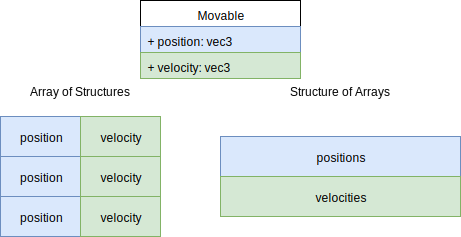
\includegraphics[width=\linewidth]{BAC-DOD1}}
	\caption{Příklad transformace pole struktur na strukturu polí.}
	\label{Fig:SOAASO}
\end{figure}

Základem \emph{DOD} je důkladná analýza aplikačních dat -- jejich obor hodnot, transformace, definice vstupních dat, požadovaný výstup atp. Často je využíváno datové struktury pole, jehož vlastnosti umožňují rychlou iteraci. Mezi výhody \emph{DOD} patří také dobrá lokalita dat a odkazů, což umožňuje efektivní využití procesorových \emph{cache}. Díky těmto vlastnostem se \emph{DOD} stále častěji používá v herním průmyslu\cite{DataOrientedDesignDice}\cite{DataOrientedDesignCppCon}.

Entitní systém navržený v této práci vychází z principů \emph{DOD} -- \emph{datově orientovaná kompozice}\cite{DODComponents}. Blíže se tímto způsobem skládání \emph{entit} zabývá sekce \ref{Chap:DOC}.

\section{Reprezentace entit}

Tato sekce obsahuje rozbor nejpoužívanějších způsobů reprezentace \emph{entit}\cite{EvolveHierarchy} a jejich \emph{chování}. Pod pojmem \emph{entita} je myšlen objekt ve virtuálním světě a \emph{chování} jsou operace, které \emph{entita} dokáže provést -- pohyb, vykreslení, kolize atp.

Jednotlivé reprezentace jsou srovnány na příkladu jednoduché 2D \emph{shoot'em up} hry. Metody jsou hodnoceny na základě složitosti implementace, návrhu s jejich použitím a výhodnosti z pohledu hardware. Závěry zde vyvozené jsou primárně zaměřené na \emph{třídní} objektově orientované jazyky (\emph{C++}, \emph{JAVA}, \emph{Python} atp.), ale částečně je lze aplikovat i na \emph{objektově orientované} programovací jazyky obecně.

\subsection{Objektově orientovaná hierarchie}

Pod pojmem \emph{objektově orientovaná hierarchie} (\emph{OOH} \cite{GameDesignPatterns}) je míněn způsob skládání nových typů entit za využití \emph{dědičnosti} a často také \emph{polymorfismu}. Příklad hierarchie, navržené pro ukázkovou 2D hru, lze vidět na obr. \ref{Fig:OOPHierarchy}. V kořenu stromu hierarchie je, v případě \emph{OOH}, bázová třída, která umožňuje uniformní skladování entit. Konkrétní entity, které existují v herním světě, jsou listy ve stromy dědičnosti.

Množina akcí entity je nastřádána průchodem stromu dědičnosti od kořene k listu, kde se konkrétní entita nachází. Existují dva často používané způsoby definice těchto akcí. První z nich je přímá definice metody v děděné třídě, tohoto je využíváno v případě akcí, které nezávisí na typu entity -- např. vykreslení. Druhým je potom využití polymorfizmu -- virtuálních metod.

\begin{figure}[H]
	\tmpframe{\includegraphics[width=\linewidth]{BAC-OOP1}}
	\caption{Příklad objektově orientované hierarchie.}
	\label{Fig:OOPHierarchy}
\end{figure}

Hierarchie dědičnosti, která je v tomto příkladě použita lze vidět na obr. \ref{Fig:OOPHierarchy} -- pouze ilustrační, pro předvedení problémů. Bázová třída \textbf{Entity} obsahuje kód pro vykreslování, dále se hierarchie dělí na entity pohyblivé a statické. Prvním problémem je umístění entit, které jsou v pozadí -- nelze do nich narazit. Dalším příkladem problémů s \emph{OOH} je přidání třídy \textbf{StationaryGun} (nepohyblivá zbraň), u které není optimální třída, ze které by měla dědit.

Pro příklad využití paměti je využit seznam pohybujících se entit, jejichž pozice musí být každý snímek hry aktualizována o jejich rychlost. Ilustrace možné organizace paměti lze vidět na obr. \ref{Fig:OOPMemory}. Hlavní seznam obsahuje ukazatele na entity, které je potřeba aktualizovat. Instance jednotlivých konkrétních typů jsou uloženy ve vlastních seznamech.

\begin{figure}
	\tmpframe{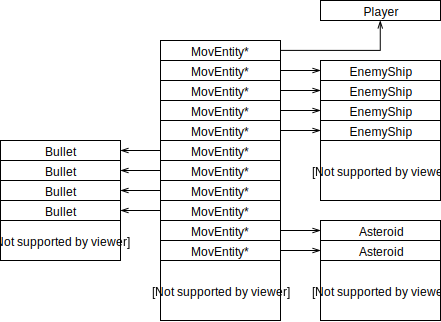
\includegraphics[width=\linewidth]{BAC-OOP2}}
	\caption{Obsah paměti u objektově orientovaných hierarchií.}
	\label{Fig:OOPMemory}
\end{figure}

Při operaci aktualizace je iterováno přes hlavní seznam ukazatelů a na každý objekt je zavolána metoda, která aktualizuje pozici o jeho rychlost. Postup práce s hlavní pamětí a \emph{cache} je následující \footnote{Postup neuvažuje různé vrstvy paměti \emph{cache} a předpokládá, že k požadovanému bloku paměti zatím nebylo přistoupeno. Velikost řádku vyrovnávací paměti je nastavena tak, aby nedošlo k překrytí paměti ukazatelů a paměti instancí.}. Prvním krokem je načtení bloku paměti o velikosti řádku vyrovnávací paměti (\emph{cache}), který obsahuje požadované ukazatele. Následuje dereference prvního z ukazatelů, která zapříčiní čtení dalšího řádků paměti, který již obsahuje iterované objekty. Ilustrace obsahu paměti \emph{cache} lze vidět na obr. \ref{Fig:OOPCache}. Díky způsobu, kterým jsou entity skládány, obsahují jednotlivé objekty kromě požadovaných informací -- pozice a rychlost -- také data, která nejsou používána. Výsledkem je neoptimální využití procesorových \emph{cache} \cite{DataOrientedDesignDice}.

\begin{figure}
	\tmpframe{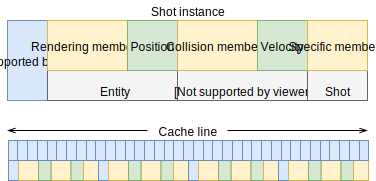
\includegraphics[width=\linewidth]{BAC-OOP3}}
	\caption{Využití procesorové \emph{cache} při použití objektově orientované entitní hierarchie.}
	\label{Fig:OOPCache}
\end{figure}

Komunikace jednotlivých částí je při použití \emph{OOH} implicitní -- pomocí \emph{public} a \emph{protected} členů. 

\pagebreak

\noindent Mezi výhody \emph{OOH} patří: 
\begin{itemize}
	\item Jednoduchá implementace.
	\item Podpora tříd zabudována do mnoha programovacích jazyků.
	\item Použití standardních návrhových metod z objektově orientovaného návrhu.
	\item Implicitní propojení a komunikace mezi děděnými částmi.
\end{itemize}

\noindent Její nevýhody jsou: 
\begin{itemize}
	\item Akumulace stavu a chování, které není nutně entitou vyžadováno.
	\item Duplikace kódu v různých větvích stromu dědičnosti.
	\item Zvyšující se složitost umisťování nových typů entit.
	\item Typy entit jsou specifikovány ve zdrojovém kódu.
	\item Statické typování \footnote{Může být výhodou v některých případech, např. optimalizace, které vykonává překladač.}, nemožnost tvorby nových typů za běhu programu.
\end{itemize}

\subsection{Objektově orientovaná kompozice}

Pod pojmem \emph{objektově orientovaná kompozice} (\emph{OOC} \cite{GameDesignPatterns}) je myšlena tvorba entit z menších částí -- komponent -- kde komponenty obsahují data i množinu proveditelných akcí. Entita je při použití \emph{OOC} kontejner, který obaluje seznam komponent (kompozice). Příklad návrhu množiny komponent lze vidět na obr. \ref{Fig:OOCHierarchy}, kontejnerovou třídou je v tomto případě \textbf{Entity}.

Množinu akcí, které lze nad entitou provést je definována komponenty, které jsou v entitě přítomny. Každá komponenta obsahuje, kromě dat, také akce, které lze nad entitou, která danou komponentu obsahuje, provést.

Tato je často používaná (\emph{composition over inheritance}) v návrhu software a je mezikrokem od \emph{objektově orientované hierarchie} k \emph{datově orientované kompozici}. 

\begin{figure}
	\tmpframe{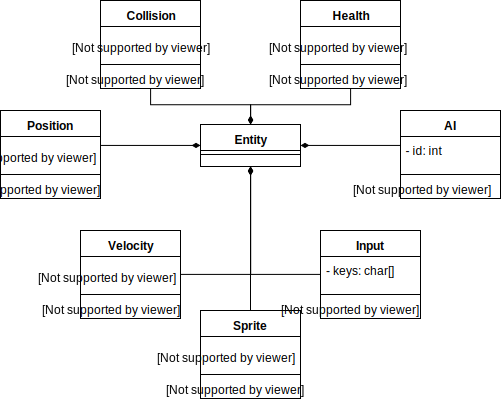
\includegraphics[width=\linewidth]{BAC-OOC1_1}}
	\caption{Příklad objektově orientované kompozice.}
	\label{Fig:OOCHierarchy}
\end{figure}

Příkladem využití těchto komponent, pro implementaci stejné množiny konkrétních entit, jako v případě použití \emph{OOH}, lze vidět na obr. \ref{Fig:OOCEntity}. Oproti využití dědičnosti se zde již lze jednoduše vyhnout problému s umístěním entit do stromu dědičnosti. Přidání typu \textbf{StationaryGun} je již také bezproblémové, díky možnosti libovolné kombinace jednotlivých komponent.

\begin{figure}
	\tmpframe{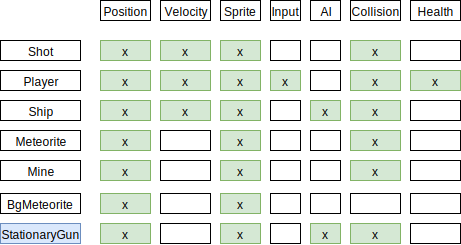
\includegraphics[width=\linewidth]{BAC-OOC1_2}}
	\caption{Využití kompozice pro tvorbu herních objektů. Konkrétní typy entit jsou zde reprezentovány řádky, jednotlivé komponenty jsou potom sloupce. Přítomnost komponenty je vyznačena znakem \uv{\emph{x}}.}
	\label{Fig:OOCEntity}
\end{figure}

Existuje mnoho způsobů, jak tuto základní myšlenku kompozice z menších částí implementovat. Jednou z možností je vyhradit pro každý typ komponenty pozici v seznamu ukazatelů \footnote{Mezi další způsoby patří mapy nebo dynamické seznamy. Možným řešením je také použití obecných ukazatelů a typových proměnných. }. V tomto návrhu je entita redukována na seznam ukazatelů, kde každá komponenta je buď přítomna (ukazatel je nastavený), nebo nepřítomna (ukazatel je \emph{NULL}). Výhodou této implementace je rychlost. Primární nevýhodou je potom neefektivní využití paměti, pro větší množství druhů komponent. Ilustraci této implementace lze vidět na obr. \ref{Fig:OOCImpl}. 

\begin{figure}
	\tmpframe{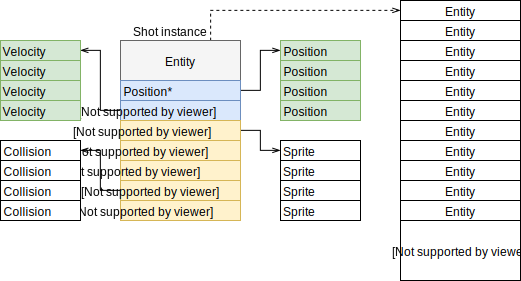
\includegraphics[width=\linewidth]{BAC-OOC2}}
	\caption{Obsah paměti u objektově orientované kompozice. Zde je entita implementována pomocí seznamu ukazatelů.}
	\label{Fig:OOCImpl}
\end{figure}

Jako příklad práce s pamětí je použita iterace nad seznamem entit, u kterých je nutno provést aktualizaci pozice, podle jejich rychlosti. V tomto příkladě je použita implementace pomocí statického seznamu ukazatelů, podle obr. \ref{Fig:OOCImpl}.

Podobně, jako u použití \emph{OOH}, je zde iterováno přes seznam, který však tentokrát obsahuje již jednotlivé instance typu \textbf{Entity} \footnote{Předpokládá se, že všechny entity obsahují komponenty typu \textbf{Position} a \textbf{Velocity}}. Využití vyrovnávací paměti, za stejných předpokladů, jako u příkladu v případě \emph{OOH}, je následující. Nejdříve je načten seznam entit a jejich ukazatelů na jednotlivé komponenty. Požadovaná operace potřebuje pouze ukazatele na komponenty typu \textbf{Position} a \textbf{Velocity}, ostatní jsou v tomto případě zbytečné \footnote{Záleží na implementaci, tuto neefektivitu je možné řešit optimalizacemi. }. Následuje přístup k požadovaným komponentám skrz ukazatele v první entitě. Tímto je načten blok paměti, pro každou komponentu, do vyrovnávací paměti. Po provedení operace nad první entitou a přístupu k dalším jsou již následující komponenty přístupné z \emph{cache}. 

\begin{figure}
	\tmpframe{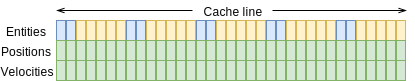
\includegraphics[width=\linewidth]{BAC-OOC3}}
	\caption{Využití procesorové \emph{cache} při použití objektově orientované kompozice.}
	\label{Fig:OOCCache}
\end{figure}

Komunikace mezi jednotlivými komponenty je při použití \emph{objektově orientované kompozice} problematické. Příkladem by mohla být \emph{umělá inteligence}, která potřebuje změnit rychlost entity. Jelikož jsou jednotlivé komponenty samostatné (\emph{encapsulation}) objekty, oddělené od ostatních komponent, které jsou součástí stejné entity, není mezi nimi možná přímá komunikace. Jedním možným řešením je přidání systému zpráv \footnote{Zprávy, ale i události jsou možným řešením.}, který má přístup k entitě, jako celku a předat odkaz na tento systém jednotlivým komponentám.

\noindent Mezi výhody \emph{OOC} patří: 
\begin{itemize}
	\item Uniformní instance všech typů entit, liší se pouze v přítomných komponentách.
	\item Lepší využití procesorových \emph{cache}.
	\item Možnost definování nových typů entit za běhu, použitím kompozice.
	\item Definice typů entit v datech.
	\item Komponenty, které entita vlastní, jsou přístupny z jednoho místa.
	\item Odstraněna duplikace kódu a akumulace nechtěného stavu.
\end{itemize}

\noindent Její nevýhody jsou: 
\begin{itemize}
	\item Složitější implementace, většinou bez podpory v programovacím jazyce.
	\item Komunikace mezi komponentami není implicitní, je nutno ji implementovat. 
\end{itemize}

\subsection{Datově orientovaná kompozice}
\label{Chap:DOC}
\todo{Popis, příklad, vyhodnocení výhod/nevýhod, komunikace}



\begin{figure}[H]
	\tmpframe{\includegraphics[width=\linewidth]{BAC-DOC1_1}}
	\caption{Příklad datově orientované kompozice.}
\end{figure}
\begin{figure}[H]
	\tmpframe{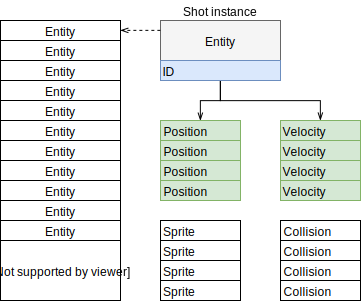
\includegraphics[width=\linewidth]{BAC-DOC2}}
	\caption{Obsah paměti u datově orientované kompozice.}
\end{figure}
\begin{figure}[H]
	\tmpframe{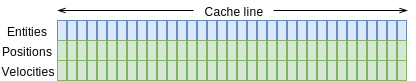
\includegraphics[width=\linewidth]{BAC-DOC3}}
	\caption{Využití procesorové \emph{cache} při použití datově orientované kompozice.}
\end{figure}
\blind[4]

ciste knoceptualni

\section{Entitní systém}
\subsection{Koncept}
\todo{Představení základní architektury návrhového vzoru - entity, komponenty, systémy}
\begin{figure}[H]
	\tmpframe{\includegraphics[width=\linewidth]{TODO-image}}
	\caption{Entita reprezentována jako řádek v databázi. \todo{Vytvořit}}
\end{figure}
\blind[5]

\subsection{Výhody zvolené reprezentace}
\todo{Lokalita dat, instrukcí. Cache. Dynamičnost, prototypování. Serializace. Embedded skriptovací jazyky.}
\blind[4]

\section{Paralelizmus}
\label{Chap:Parallelism}
\todo{Důležitost, hardware - cache, popis možností paralelizace.}
\blind[2]
\begin{figure}[H]
	\tmpframe{\includegraphics[width=\linewidth]{TODO-image}}
	\caption{Paralelizmus uvnitř systémů. \todo{Vytvořit}}
\end{figure}
\blind[1]
\begin{figure}[H]
	\tmpframe{\includegraphics[width=\linewidth]{TODO-image}}
	\caption{Paralelizmus na úrovni systémů. \todo{Vytvořit}}
\end{figure}
\blind[1]
%https://software.intel.com/en-us/articles/designing-the-framework-of-a-parallel-game-engine

\chapter{Návrh entitního systému}
\todo{Co by to melo umet, priority}

\section{Přehled a komunikace}
\todo{Postup seznámení s návrhem top -> down}
\begin{figure}[H]
	\tmpframe{\includegraphics[width=\linewidth]{TODO-image}}
	\caption{Návrhový diagram komponentního systému. \todo{Vytvořit}}
\end{figure}
\blind[1]
\todo{High-level design, propojení. Universe, action-cache.}
\begin{figure}[H]
	\tmpframe{\includegraphics[width=\linewidth]{TODO-image}}
	\caption{Přehled návrhu komponentního systému a komunikace mezi jeho částmi. \todo{Vytvořit - HLB diagram}}
\end{figure}
\blind[3]

\section{Komponenty a jejich nosiče}
\todo{Komponenta POD. Trivial constructor, copy. Paměť a typy nosičů. Typy komponent - tag, normal.}
\blind[4]

\section{Systémy a skupiny}
\todo{Volnost použití systémů. Uživatelem definované chování. Filtry - require, reject. Cache pomocí skupin entit.}
\blind[5]

\section{Reprezentace entit}
\todo{Entita, id, generace. Alternativy a důvody.}
\blind[3]

\section{Paralelní přístup}
\todo{Podporované způsoby paralelizace, návrh, zdůvodnění. Entity paralellization. System parallelization. Diskuze na téma, zda je paralelní přístup potřeba.}
\blind[5]

\section{Tok řízení}
\todo{Popsat předpokládaný tok řízení, jak se bude používat. Registrace. Iterace. Refresh.}
\begin{figure}[H]
	\tmpframe{\includegraphics[width=\linewidth]{TODO-image}}
	\caption{Digram toku řízení komponentního systému. \todo{Vytvořit - Control flow diagram}}
\end{figure}
\blind[3]


\chapter{Implementace}
\todo{Shrnutí návrhu}
\blind[2]

\section{Použité knihovny a přenositelnost}
\todo{zduvodneni pouziti c++ Zdůvodnění nepoužití knihoven. C++14, Linux, Windows. Header-only}
\blind[2]

\section{Komponenty}
\todo{Rekapitulace vlastností, které komponenta musi splnit. Registrace, generování identifikátorů. Uživatelské nosiče}
\blind[3]

\section{Systémy a skupiny}
\todo{Super třída, filtry, přístup - iterace. Přidání systému, volitelná skupina - added/removed.}
\blind[3]

\section{Správa entit}
\todo{Potřebné informace, implementace, datové struktury, optimalizace}
\blind[3]

\section{Obnovovací fáze}
\todo{Pořadí refresh. Obnovení aktuality skupin.}
\blind[2]

\section{Podpora paralelizmu}
\todo{2 způsoby paralelizmu - dělení skupin, change-sety}
\blind[3]


\chapter{Použití knihovny}

\section{Demo hra}
\todo{Popis principů hry}
\blind[1]

\section{Návrh}
\todo{Komponentní návrh}
\blind[3]

\section{Zhodnocení}
\todo{Výkon, návrh, jednoduchost}
\blind[3]

\chapter{Vyhodnocení}
\todo{Shrnutí, popis co bude v této kapitole}
\blind[1]

\section{Testování knihovny}
\todo{Unit testing, benchmarky}
\blind[2]

\section{Testované sestavy}
\todo{Hardware sestavy - PC, notebook. Tabulka identifikace}
\blind[1]

\section{Výkonnostní testy}
\todo{Výkon při různých zatíženích - procenta přidaných/odebraných. Grafy.}
\blind[1]
\todo{Porovnání nosičů komponent. Grafy.}
\blind[1]
\todo{Seriové vs paralelní - počet vláken. Grafy.}
\blind[1]

\section{Porovnání}
\todo{Výkonostní porovnání oproti jiným ECS knihovnám, Unity? Grafy.}
\blind[2]

\subsection{Implementace}
\todo{Použité knihovny, základní popis implementace}
\blind[2]

\subsection{Výsledek}
\todo{Poznatky a výsledky získané ze hry. Grafy?}
\blind[2]


\chapter{Závěr}
\todo{Využití komponentních systémů a aktuální stav} 
\blind[1]
\todo{Návrh, prototypy, priority} 
\blind[1]
\todo{Implementace, rozšiřitelnost, přenositelnost}
\blind[1]
\todo{Experimenty, srovnání, demo hra}
\blind[1]
\todo{Možnosti rozšíření}
\blind[1]

%\begin{figure}
%	\tmpframe{\includegraphics[width=\linewidth]{TODO-image}}
%	\caption{Obrazek \todo{Obrazek}}
%\end{figure}

%=========================================================================
